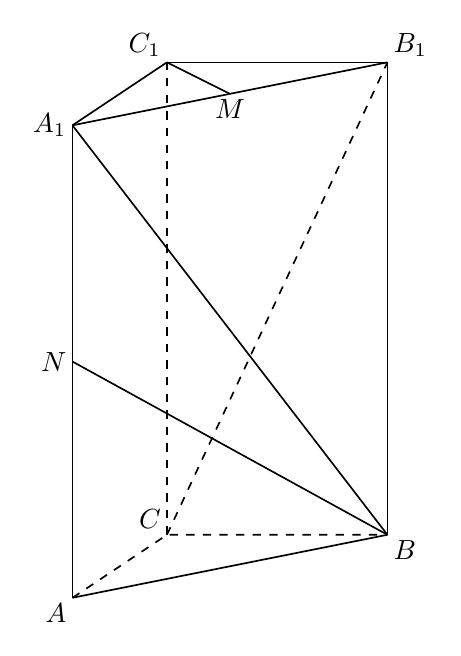
\begin{tikzpicture}[x=1cm,y=1cm,font=\normalsize,
  geometry edge/.style={line width=.6pt},
  geometry node/.style={font=\normalsize,inner sep=2pt}]
\coordinate (A) at (0,0);
\coordinate (B) at (4,0.8);
\coordinate (C) at (1.2,0.8);
\coordinate (A1) at (0,6);
\coordinate (B1) at (4,6.8);
\coordinate (C1) at (1.2,6.8);
\coordinate (M) at (2,6.4);
\coordinate (N) at (0,3);
% solid base/laterals
\draw[geometry edge] (A)--(B);
\draw[geometry edge] (A)--(A1);
\draw[geometry edge] (B)--(B1);
\draw[geometry edge] (A1)--(B1);
% solid top triangle + median
\draw[geometry edge] (C1)--(B1);
\draw[geometry edge] (A1)--(C1);
\draw[geometry edge] (C1)--(M);
% solid diagonals
\draw[geometry edge] (A1)--(B);
\draw[geometry edge] (N)--(B);
% hidden base/lateral/diagonal
\draw[geometry edge,dashed] (A)--(C)--(B);
\draw[geometry edge,dashed] (C)--(C1);
\draw[geometry edge,dashed] (C)--(B1);
\node[geometry node,below left] at (A) {$A$};
\node[geometry node,below right] at (B) {$B$};
\node[geometry node,above left] at (C) {$C$};
\node[geometry node,left] at (A1) {$A_{1}$};
\node[geometry node,above right] at (B1) {$B_{1}$};
\node[geometry node,above left] at (C1) {$C_{1}$};
\node[geometry node,below] at (M) {$M$};
\node[geometry node,left] at (N) {$N$};
\end{tikzpicture}